\documentclass{article}

\usepackage{fullpage}
\usepackage{url}
\usepackage{verbatim}
\usepackage{graphicx}
\usepackage{parskip}
\usepackage{pdfpages}

\begin{document}

% The common requirement for all project is that the students in each group need to make use in their design project any method or combination of methods of material taught in the course (or closely related to it) to solve the proposed problem or improve on an existing solution. These are the required deliverables
% A report of 20 to 25 pages needs to be provided with these sections:

\section{Abstract}

% Abstract

\section{Problem Statement and Solution Motivation}
Wearable technology, such as smartwatches, are poised to become a ubiquitous consumer product. According to businessinsider.com, smartwatches sales are projected to reach 90 million units by 2018 (http://www.businessinsider.com/global-smartwatch-sales-set-to-explode-2014-3). Many user interface paradigms still need to be rethought for these devices to accommodate their small screens and limited input methods. 

\begin{figure}[ht!]
  \centering
  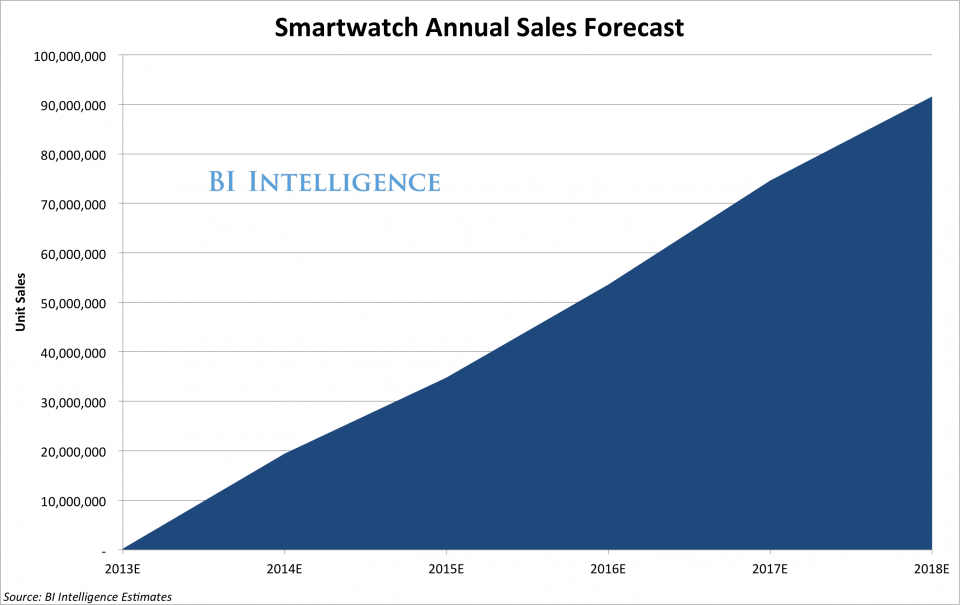
\includegraphics[width=90mm]{smartwatch.png}
  \caption{Smartwatch Annual Sales Projection \label{overflow}}
\end{figure}

Currently, these devices rely mostly on touch input and voice control. Touch input is usually effective, but due to the small form factor, a significant portion of the screen is often obscured by the user's finger. Voice control can be used to complete more complex actions that might be tedious to complete using only touch input, but voice commands are not always practical. They may be less effective in noisy environments, or users might feel uncomfortable using them in public places due to issues with privacy and social acceptance.

Hand and arm gestures could be used to augment existing input paradigms. Though less expressive than voice commands, hand and arm movements are relatively private and they are a natural way to communicate with the environment. There are presently no publicly available gesture recognition solutions for off-the-shelf smartwatches, though theories and interface ideas have been prototyped with other sensors such as Microsoft Kinect or custom ultra-sound detection systems. The potential applications of this technology are far-reaching, from seamless control of Internet-of-things devices to accessibility for visually impaired users.

We have acquired a LG G Watch R and a Nexus 5 phone to record gesture data via a simple, custom-built Android application. Data collected from the watch's accelerometer will be used to train a neural network to classify a set of simple gestures. We will compare the accuracy and performance of our classifier against similar gesture recognition systems in the research community.

\section{Theoretical Background Material}
Our work is inspired by two works in particular. First, there is the famous "Learning Representations by Back-Propagating Errors" paper that first introduced the back propagation algorithm. Second, there is "Gestures without Libraries, Toolkits, or Training: A \$1 Recognizer for User Interface Prototypes". The former lays the groundwork for our solution and the latter provided motivation for the problem domain. 

\subsection{Backpropagation}
Backpropagation has become a common method for training neural networks. Before its formulation,  there was no way to provide a measure of accuracy for hidden layers in neural networks. 

It is most often used in the supervised learning process as it requires the expected labelling for a set of inputs.  Before the formulation of this algorithm there

\subsection{\$1 Recognizer}s

% Theoretical background material with references

\section{Solution}

% Present your solution using tool(s) learned in class (or something related)

\section{Results}

% Results: Analysis and comparison if any

\section{Conclusion}

% Conclusion

\section{References}
\begin{itemize}
\item Orr, Genevieve B. "Error Backpropagation." Error Backpropagation. Williamette University, n.d. Web. 02 Apr. 2015.
\item Rumelhart, D. E., Hinton, G. E., and Williams, R. J. Learning representations by back-propagating errors. Nature, 323, 533--536 [pdf]
\item Wobbrock, J.O., Wilson, A.D. and Li, Y. (2007). Gestures without libraries, toolkits or training: A $1 recognizer for user interface prototypes. Proceedings of the ACM Symposium on User Interface Software and Technology (UIST '07). Newport, Rhode Island (October 7-10, 2007). New York: ACM Press, pp. 159-168.

\end{itemize}
% References

\end{document}
